\section{Reflex Enterprise Architecture}

\label{sec:architecture}

\subsection{Stack Overview}

The Reflex Enterprise stack implements the Chatman Equation through four integrated layers:

\begin{center}
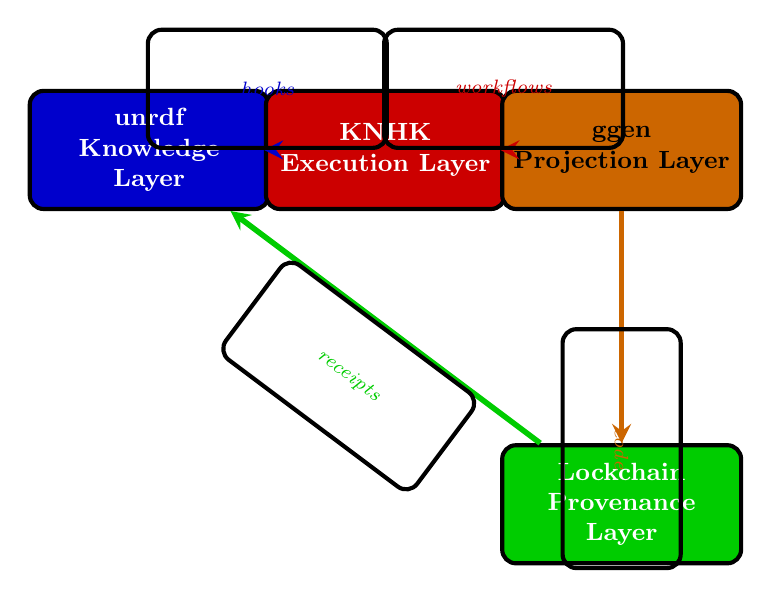
\begin{tikzpicture}[
    node distance=3cm and 4cm,
    every node/.style={rectangle, rounded corners=5pt, minimum width=3cm, minimum height=1.5cm, text centered, text width=2.8cm, font=\small\bfseries, draw=black, line width=1.5pt},
    arrow/.style={->, >=stealth, thick, line width=2pt},
    label/.style={font=\scriptsize\itshape, midway, sloped}
]
    \node[fill=blue!80!black, text=white] (unrdf) {unrdf\\Knowledge Layer};
    \node[fill=red!80!black, text=white, right of=unrdf] (knhk) {KNHK\\Execution Layer};
    \node[fill=orange!80!black, text=black, right of=knhk] (ggen) {ggen\\Projection Layer};
    \node[fill=green!80!black, text=white, below of=ggen, yshift=-1.5cm] (lockchain) {Lockchain\\Provenance Layer};
    
    \draw[arrow, blue!80!black] (unrdf) -- node[label, above] {hooks} (knhk);
    \draw[arrow, red!80!black] (knhk) -- node[label, above] {workflows} (ggen);
    \draw[arrow, orange!80!black] (ggen) -- node[label, right] {code} (lockchain);
    \draw[arrow, green!80!black] (lockchain) -- node[label, below] {receipts} (unrdf);
\end{tikzpicture}
\end{center}

\subsection{unrdf: Knowledge Layer}

\textbf{unrdf} provides the bounded autonomic layer of Reflex—Knowledge Hooks that detect, validate, and enforce enterprise rules via \RDF{} and SHACL. Each hook enforces invariants and emits Merkle receipts into Lockchain for full traceability.

\textbf{Components}:
\begin{itemize}
    \item \textbf{Knowledge Hooks}: Policy-bound programs over \RDF{} knowledge graphs
    \item \textbf{SHACL Validation}: Shape constraint checking at ingress
    \item \textbf{SPARQL Queries}: Boolean queries (ASK) and data queries (SELECT)
    \item \textbf{OTEL Integration}: Full OpenTelemetry spans for observability
    \item \textbf{Lockchain Integration}: Cryptographic receipt generation
\end{itemize}

\textbf{SLO}: Warm path $\leq 500$ ms for hook service time (P99).

\subsection{KNHK: Execution Layer}

\textbf{KNHK} implements the measurement operator $\mu(O)$ in the Hot Path domain, producing deterministic projections ($A = \mu(O)$) with $\leq 2$ ns evaluation latency per rule. Every cycle concludes with guard validation and receipt issuance, ensuring that all runtime actions are mathematically traceable and verifiable.

\textbf{Components}:
\begin{itemize}
    \item \textbf{Hot Path (C)}: $\leq 8$ ticks ($\leq 2$ ns) for rule checks (ASK, COUNT, COMPARE, VALIDATE)
    \item \textbf{Warm Path (Rust)}: $\leq 500$ ms for workflow orchestration and ETL
    \item \textbf{Cold Path (Erlang/SPARQL)}: $\leq 500$ ms for complex queries and reasoning
    \item \textbf{43/43 Pattern Coverage}: All Van der Aalst workflow patterns as deterministic operators
    \item \textbf{Guard Enforcement}: Ingress guards $H$ enforce legality, budgets, chronology, causality
\end{itemize}

\textbf{SLO}: Hot path $\leq 2$ ns (P99), warm path $\leq 500$ ms (P99), cold path $\leq 500$ ms (P99).

\subsection{ggen: Projection Layer}

\textbf{ggen} operationalizes bounded regeneration. It reprojects ontology schemas into code across multiple languages (Rust, TypeScript, Python) until no measurable drift exists between ontology triples and generated artifacts. Each regeneration cycle produces verifiable receipts ensuring determinism and reproducibility across all runtime tiers.

\textbf{Components}:
\begin{itemize}
    \item \textbf{Ontology Compilation}: \RDF{} ontologies compiled to executable schemas
    \item \textbf{Multi-Language Projection}: Code generation across Rust, TypeScript, Python
    \item \textbf{Bounded Regeneration}: Iterates until schema drift $\leq 0.5\%$ or receipt delta $< 10^{-3}$
    \item \textbf{Receipt Generation}: Meta-receipts for each regeneration cycle
\end{itemize}

\textbf{SLO}: Regeneration halts when drift $\leq \varepsilon$ (typically $0.5\%$).

\subsection{Lockchain: Provenance Layer}

\textbf{Lockchain} provides SHA3-256 Merkle chains for all actions. Replays must reproduce $\mathrm{hash}(A) = \mathrm{hash}(\mu(O))$ within tolerance. Every action produces a receipt that cryptographically verifies the execution path.

\textbf{Components}:
\begin{itemize}
    \item \textbf{Merkle Chains}: SHA3-256 cryptographic hashing
    \item \textbf{Receipt Storage}: Git-based immutable audit logs
    \item \textbf{Verification}: Independent recomputation must reproduce hash within $10^{-3}$ tolerance
    \item \textbf{Provenance Tracking}: Full lineage from ontology to action
\end{itemize}

\textbf{SLO}: Receipt delta $< 10^{-3}$ within tolerance.

\subsection{Integration Flow}

The Reflex Enterprise stack operates as a closed loop:

\begin{enumerate}
    \item \textbf{Ingress}: Change $\Delta O$ detected in knowledge graph
    \item \textbf{Hook Evaluation}: unrdf hooks evaluate invariants and guards
    \item \textbf{Workflow Execution}: KNHK executes workflow patterns (43/43 patterns)
    \item \textbf{Code Projection}: ggen projects ontology changes to code (if needed)
    \item \textbf{Receipt Generation}: Lockchain produces cryptographic receipt
    \item \textbf{Verification}: Receipt verifies $\mathrm{hash}(A) = \mathrm{hash}(\mu(O))$
\end{enumerate}

\subsection{Three-Tier Performance Architecture}

The KNHK execution layer implements a three-tier performance architecture. The \textbf{Hot Path (C)} executes rule checks within $\leq 8$ ticks ($\leq 2$ ns), providing deterministic evaluation for simple operations. The \textbf{Warm Path (Rust)} handles orchestration and ETL within $\leq 500$ ms, managing batch operations and enterprise integrations. The \textbf{Cold Path (Erlang/SPARQL)} processes complex queries within $\leq 500$ ms, supporting historical reconciliation and reasoning. All paths enforce guards at ingress, produce receipts, and maintain bounded execution guarantees.

\begin{center}
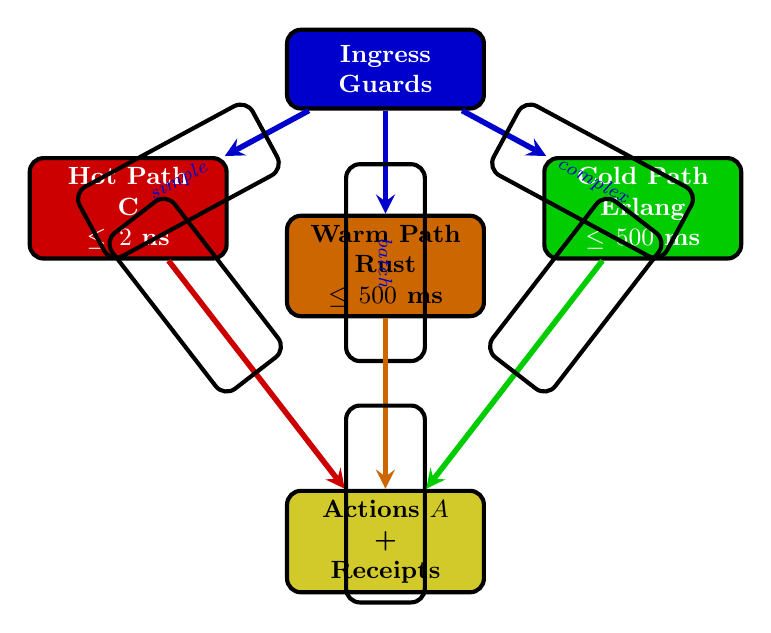
\begin{tikzpicture}[
    node distance=2.5cm and 1.5cm,
    every node/.style={rectangle, rounded corners=5pt, minimum width=2.5cm, minimum height=1cm, text centered, text width=2.2cm, font=\small\bfseries, draw=black, line width=1.5pt},
    arrow/.style={->, >=stealth, thick, line width=2pt},
    label/.style={font=\scriptsize\itshape, midway, sloped}
]
    \node[fill=blue!80!black, text=white] (ingress) {Ingress\\Guards};
    \node[fill=red!80!black, text=white, below left of=ingress, xshift=-1.5cm] (hot) {Hot Path\\C\\$\leq 2$ ns};
    \node[fill=orange!80!black, text=black, below of=ingress] (warm) {Warm Path\\Rust\\$\leq 500$ ms};
    \node[fill=green!80!black, text=white, below right of=ingress, xshift=1.5cm] (cold) {Cold Path\\Erlang\\$\leq 500$ ms};
    \node[fill=yellow!80!black, text=black, below of=warm, yshift=-1cm] (actions) {Actions $A$\\+\\Receipts};
    
    \draw[arrow, blue!80!black] (ingress) -- node[label, left] {simple} (hot);
    \draw[arrow, blue!80!black] (ingress) -- node[label, right] {batch} (warm);
    \draw[arrow, blue!80!black] (ingress) -- node[label, right] {complex} (cold);
    \draw[arrow, red!80!black] (hot) -- node[label, left] {} (actions);
    \draw[arrow, orange!80!black] (warm) -- node[label, right] {} (actions);
    \draw[arrow, green!80!black] (cold) -- node[label, right] {} (actions);
\end{tikzpicture}
\end{center}

\begin{tcolorbox}[colback=blue!5!white,colframe=blue!75!black,title=\textbf{Stack Economics: Cost per Decision}]
\textbf{Hot-path cost}: Amortized compute + receipt write (micro-cents per decision).

\textbf{Warm-path cost}: Batch orchestration + connectors (sub-millisecond amortization).

\textbf{Cold-path cost}: Complex query processing + historical reconciliation (millisecond amortization).

\textbf{Total cost}: Proportional to evaluated rules, not meeting hours or headcount.
\end{tcolorbox}

\subsection{Guard Enforcement}

All actions are guard-verified ($\mu \adjoint H$) at ingress. Guards enforce \textbf{legality} by ensuring actions comply with legal and regulatory requirements, \textbf{budgets} by respecting financial constraints, \textbf{chronology} by preserving temporal ordering (no retrocausation), and \textbf{causality} by respecting causal dependencies. No action executes without guard verification. All guards are enforced at ingress, not scattered throughout code.

\subsection{Receipt Schema}

Every action produces a receipt $R = (\mathrm{actor}, \mathrm{delta}, \mathrm{guard\_set}, \mathrm{SLO}, \mathrm{merkleRoot})$ where $\mathrm{actor}$ is the entity that triggered the action (system, user, or hook), $\mathrm{delta}$ is the change $\Delta O$ that triggered the action, $\mathrm{guard\_set}$ are the guards $H$ that were enforced, $\mathrm{SLO}$ is the service level objective (hot/warm/cold path), and $\mathrm{merkleRoot}$ is the SHA3-256 Merkle root for tamper detection. Receipts enable end-to-end recomputation and audit. Independent recomputation must reproduce $\mathrm{hash}(A) = \mathrm{hash}(\mu(O))$ within $10^{-3}$ tolerance; otherwise the claim is falsified.

